\section{Beginner's Algorithm}
\label{sec:beginner}
This section describes the easiest algorithm to remember for a human solver.
The algorithm is divided into five different steps. Once the algorithm has been memorized, it is easy to recognize which step of the algorithm has been reached, so the correct move sequence can be applied. 
Beginner's algorithm can however be made more efficient by remembering another rather similar move sequence for a few of the steps. 
Despite of this beginner's algorithm is twist-wise quite inefficient, because the purpose of the move sequences is to reach the next step instead of reaching the solved state and thereby taking a solving detour. 

\subsection{Step 1 - Getting the Cross}\label{sub:step1}
\begin{wrapfigure}{R}{0.4\textwidth}
\vspace{-8mm}
\begin{center}
	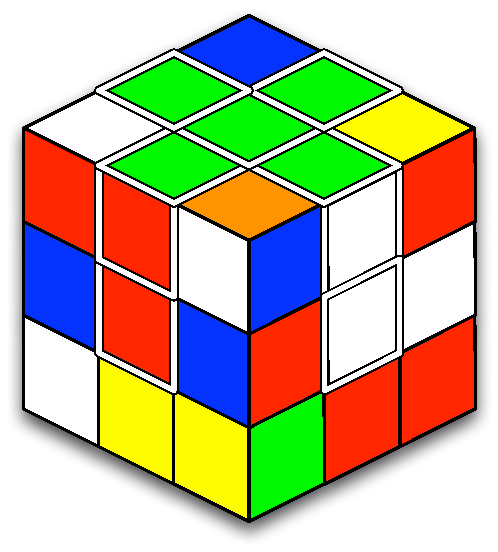
\includegraphics[width=0.28\textwidth]{input/pics/1FLcross.pdf}	
\end{center}
\caption{\myCaption{A first layer cross on the green face}}
%\vspace{-12mm}
\label{fig:1FL-cross}
\end{wrapfigure}
The first step of beginner's algorithm \cite{beginner} is to get a cross on any face. 
Getting a cross on a face means to align the \facelet{}s next to the center \facelet{}, so that all of the aligned \facelet{}s are of the same color. 
At the same time the used edge \cpiece{}s should have the same color of the center \facelet{}s on each of the two faces on which they are on. See figure \ref{fig:1FL-cross} for a correctly assembled cross on the green face.



The face on which the cross is being assembled is set to be the up face. 
An edge \cpiece{} that consists of the same colors as the center \cpiece{} of the up face and the center \cpiece{} of the front face is placed in the bottom of the front face. 
With two twists of the front face the edge \cpiece{} is positioned correctly in the cross. 
If the edge \cpiece{} is orientated correctly the \cube{} is turned and the process is repeated until the cross is assembled. 
However if the \cpiece{} is orientated in the wrong way the following move sequence will change its orientation without ruining any part of the cross that may already be assembled: \\

\m{F' U L' U'} or \m{F U' R U}

\subsection{Step 2 - Completing the First Layer}\label{sub:step2}
When the cross is completed the next step is to position the corner \cpiece{}s of the first layer correctly. The first layer is set as the down face. 
A corner with a \facet{} of the color of the down face is positioned directly above its correct  position. 
The correct position is between the three faces that have the same colors as the three \facet{}s of the corner \cpiece{}. 

\begin{wrapfigure}{R}{0.4\textwidth}
\vspace{-8mm}
\begin{center}
	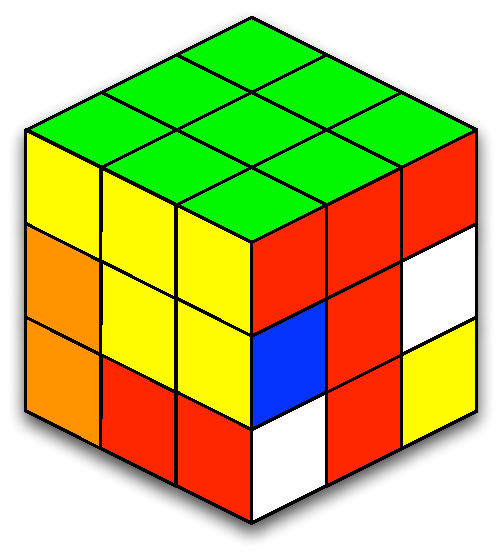
\includegraphics[width=0.28\textwidth]{input/pics/2FL.pdf}	
\end{center}
\caption{\myCaption{The first layer completed. Note that the first layer is up.}}
\label{fig:2FL}
\end{wrapfigure}


Once the \cpiece{} is above its correct position, the \cube{} should be viewed in such an angle that the \cpiece{} is in the upper right corner of the front face, the following move sequence is repeated until the corner \cpiece{} is orientated and positioned correctly (see figure \ref{fig:2FL}): \\

\m{R' D' R D} \\

If the \cpiece{} is above the correct position the algorithm twists the corner clockwise and positions it in the correct position. If the \cpiece{} is in the correct position the algorithm positions the \cpiece{} above the correct position. The maximum number of repetitions until the \cpiece{} is orientated and positioned correctly is five, because the \cpiece{} can be two twists away from its correct orientation. 
The move sequence can be performed inverted which twists the corner counterclockwise and looks as follows: \\

\m{D' R' D R} \\

If the correct move sequence is used the maximum number of repetitions is three. If number of twists and time used is not of importance it is only necessary to remember one of them.


\subsection{Step 3 - Completing the Second Layer}\label{sub:step3}
Now the \cube{} is turned, so the first layer will be down. 
The purpose of this step is to position the four edge \cpiece{}s belonging to the second layer correctly. 
The move sequence used in this step either swaps the top edge \cpiece{} of the front face with the left or right edge \cpiece{}. 
The edge \cpiece{} that needs to be positioned must have a \facelet{} that is of the same color as the front face. This \facelet{} must be on the front face. 
The \cube{} needs to be turned to get the correct front face, and then the up face is twisted in order to get the correct \cpiece{} on the front face. 
There is however a difference in which of the two faces is used as the front face, because if the wrong face is used as front face the \cpiece{} will only be positioned correctly but not orientated correctly. 
That \facelet{} of the edge towards the front face must be of the same color as the front face. 
If the edge \cpiece{} is to be swapped with the right edge \cpiece{} of the front face the following move sequence is used: \\

\m{U R U' R' U' F' U F} \\

If the \cpiece{} is to be swapped with the left edge \cpiece{} of the front face the following move sequence is used: \\

\begin{wrapfigure}{R}{0.4\textwidth}
\vspace{-5mm}
\begin{center}
	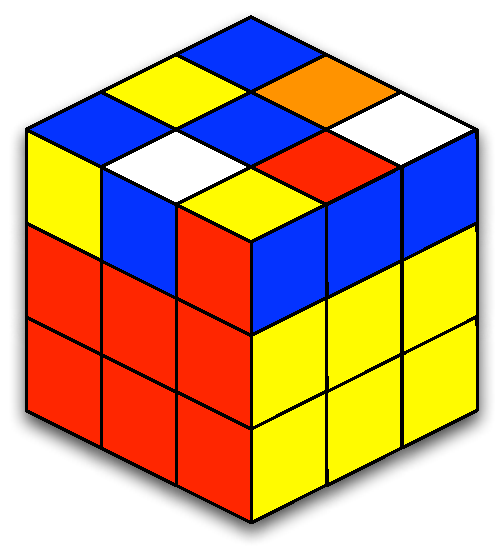
\includegraphics[width=0.28\textwidth]{input/pics/3F2L.pdf}	
\end{center}
\caption{\myCaption{The first two layers completed}}
\vspace{-5mm}
\label{fig:3F2L}
\end{wrapfigure}

\m{U' L' U L U F U' F'} \\


If none of the edge \cpiece{}s who belong to the second layer are in the third layer and the first two layers are still not completed. 
This occurs if the edges are all in the second layer but not positioned or orientated correctly. 
One of the move sequences can be used to swap an edge \cpiece{} from the third layer with one of the edges in the second layer which is not positioned or orientated correctly.
Now the edge \cpiece{} belonging to the second layer can be moved to its correct position. See figure \ref{fig:3F2L}.





\subsection{Step 4 - Getting the Last Layer Cross}\label{sub:step4}
%%%Step 4 is divided into 4 step? Perhaps substeps instead.
Solving the last layer is divided into four substeps. The order of these steps can be different and still yield the same result. We start out by getting the cross in the last layer (see figure \ref{fig:cross:6LLcross3}), which is the same as the cross on the first layer. The move sequence used is however different. The only move sequence used in this step is the following: \\

\m{F R U R' U' F'} \\

Besides remembering the move sequence it is also important to know how the \cube{} should be turned.

If the up face colors form a line (see figure \ref{fig:cross:5LLcross2}). The \cube{} can be turned until the line forms a horizontal line. If the move sequence then is performed, the cross will be formed.

\begin{figure}[htb]
	\centering
		\subfloat[\myCaption{The up face colors form the opposite L.}]{\label{fig:cross:4LLcross1}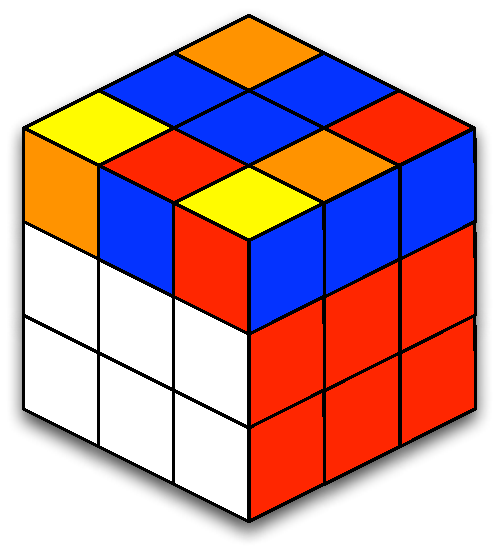
\includegraphics[width=0.28\textwidth]{input/pics/4LLcross1.pdf}}
		\hspace{0.02\textwidth}
		\subfloat[\myCaption{The up face colors form the horizontal line.}]{\label{fig:cross:5LLcross2}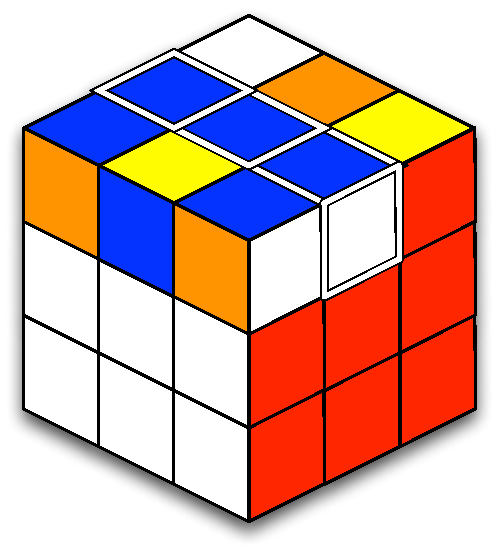
\includegraphics[width=0.28\textwidth]{input/pics/5LLcross2.pdf}}
		\hspace{0.02\textwidth}
		\subfloat[\myCaption{The up face colors form the cross.}]{\label{fig:cross:6LLcross3}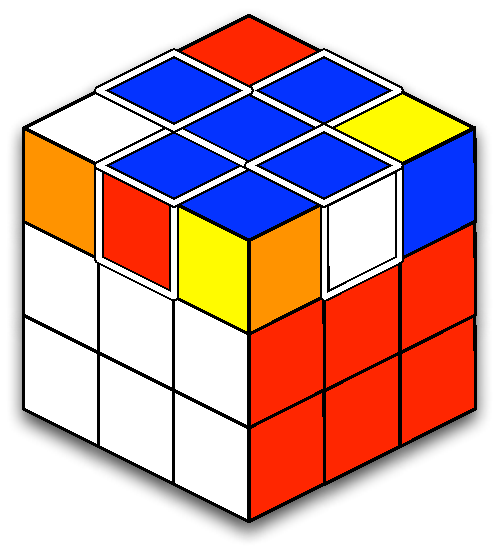
\includegraphics[width=0.28\textwidth]{input/pics/6LLcross3.pdf}}
		\caption{\myCaption{The steps in the completion of the last layer cross}}
		\label{fig:cross}
\end{figure}

If the up face colors form an opposite ``L'' (see figure \ref{fig:cross:4LLcross1}) with the up face colors the move sequence will form the line. 
The \cube{} must be orientated with the opposite ``L'' in the back left corner of the \cube{}. 

If the up face colors do not form the opposite ``L'' the line or the cross (see figure \ref{fig:3F2L}), the move sequence will form the opposite ``L''.

\begin{wrapfigure}{R}{0.4\textwidth}
\begin{center}
	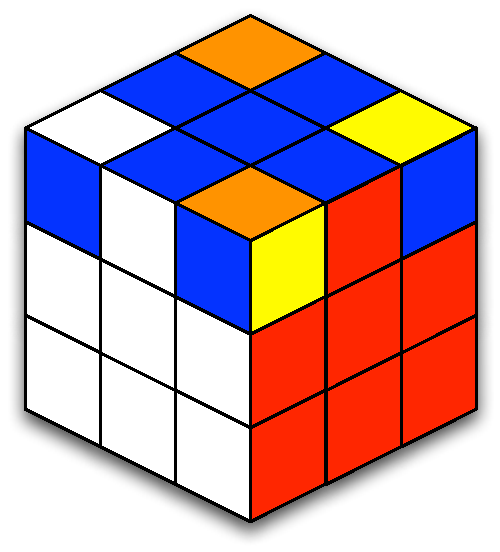
\includegraphics[width=0.28\textwidth]{input/pics/7LLedges.pdf}	
\end{center}
\caption{\myCaption{The correct orientated last layer cross.}}
\label{fig:7LLedges}
\end{wrapfigure}


To orientate the cross correctly there is one move sequence to remember: \\

\m{R U R' U R U2 R'} \\

Again it is important to know how to turn the \cube{}. By twisting the upper layer it is possible to position the upper layer so it either has two edge pieces next to each other or directly across from each other.

If the correct edge \cpiece{}s are next to each other. 
The \cube{} must be turned so it has a correct edge \cpiece{} on the back face and a complete face on the right face. 
The move sequence will then make it possible to twist the up layer so that all the edge pieces are correctly positioned and orientated (see figure \ref{fig:7LLedges}). 

If the correct edge pieces are across each other the move sequence can be performed a single time to get two edge pieces next to each other. 


\subsection{Step 5 - Completing the Last Layer}\label{sub:step5}
The purpose of this step is to position and orientate the corners correctly. Firstly the corners must be positioned correctly. To do so there are two move sequences to remember -- one for rotating three corners clockwise and one for rotating them counterclockwise. It is however only necessary to remember one of them and repeat that one until the corners are positioned correctly, if the number of twists is unimportant to the solver. \\
\\
\m{U R U' L' U R' U' L}
\\
This move sequence will rotate the corners counterclockwise.
\\
\\
\m{U' L' U R U' L U R'}
\\
This move sequence will rotate the corners clockwise.
\\
\\
The orientation is again important to position the corners. If one of the corners already is positioned correctly. That corner is chosen not to be moved. 

If the three other corners need to be moved counterclockwise. The correct corner is positioned as the front right corner. The move sequence will then position the corners correctly.

If the three other corners need to be moved clockwise. The correct corner is positioned as the front left corner. The move sequence will then position the corners correctly.

If there are no correct corners. One of the two move sequences above performed once will yield a correctly positioned corner \cubie{}.

\begin{wrapfigure}{R}{0.4\textwidth}
\begin{center}
	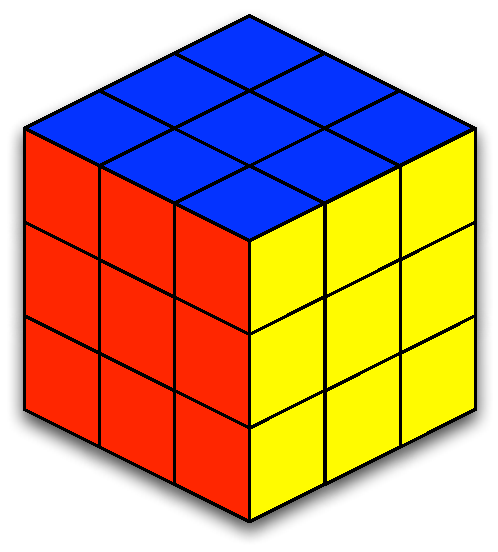
\includegraphics[width=0.28\textwidth]{input/pics/8done.pdf}	
\end{center}
\caption{\myCaption{The solved cube -- $e$}}
\label{fig:8done}
\end{wrapfigure}

To orientate the corners correctly the move sequence from orientating the corners in the first layer is used: \\

\m{R' D' R D} \\

Instead of turning the whole \cube{} to the next corner, the \cube{} is locked on one face. 
When going to solve the next corner \cubie{} the upper layer is twisted until the incorrect corner is positioned at the front-right corner \cubicle{} of the \cube{} and the move sequence is repeated. 
The \cube{} is now solved as seen on figure \ref{fig:8done}. 